\chapter{Background}
\label{background}



In this chapter, we introduce several representative cognitive radio networks, which have open questions to be answered in the following chapters.
As tool to solve the problem, game model and optimization techniques are introduced.

\section{Cognitive radio networks}
We introduce two types of cognitive radio networks, which contains the problems we will tackle in this dissertation.

\subsection{Cognitive Radio Ad Hoc Network}
%An ad hoc network is a decentralized paradigm of wireless network, which consists of a collection of autonomous mobile users which communicate over wireless links.

%Efficient distributed algorithms are needed to determine network organization, link scheduling, and routing.

CRAHN is composed with autonomous mobile cognitive radio users which work 
CRAHN is one mobile ad hoc network, whereas each mobile user has cognitive ability for spectrum access~\cite{Akyildiz09}.
Mobile users in CRAHN work with overlay spectrum sharing paradigm, thus need to determine which channels are available to use with spectrum sensing, either cooperatively with neighbour users or individually.
Mobile users have different knowledge of spectrum availability, which poses new challenges in addition to the ones for the management of mobile ad hoc network.
CRAHN can usually be represented by an undirected graph $G$.
Cognitive radio users constitute the vertices, the edge between two vertices is decided not only by the distance, propagation and attenuation properties between the two vertices, but also the spectrum availability on both vertices, \ie when they can decode the received signal from each other correctly, and there is common channel available between them on which communication is conducted, then an bidirectional edge is available on graph $G$.
As to ad hoc network, the graph is constant when users are static.
As to cognitive radio ad hoc network, due to primary users' activity, an edge between two vertices is decided by the fact that whether the two vertices can simultaneously access the same licensed channel.
Hence, the corresponding graph is dynamic under primary users' operation, which imposes extra difficulties on network organization, routing and many other network functionalities.

As a versatile and flexible network infrastructure, CRAHN is comparatively easy to implement and operate, thus CRAHN is proposed to apply in many scenarios~\cite{Akyildiz09}.
There are several open issues for CRAHN.
For instance, a robust architecture against the network dynamics caused by user' mobility, primary users' activity is still due.
It is challenging for CRAHN to meet the QoS criteria withe the spatial and temporal temporal availability of spectrum~\cite{Mansoor2014}.




%\subsection{IEEE 802.22 Standards}
%\label{ieee80222}%XXXXXXXXXXXXXX clearly statement, regulations of FCC, ECC, 802.22 XXXXXXXXXXXXXXXXXXXX
%%%XXXXXXXXXXXXXXXXXXXXXXXXXXXX   paper: IEEE 802.22: The First Cognitive Radio Wireless Regional Area Networks (WRANs) Standard
%IEEE 802.22~\cite{802.22} is the standard for Wireless Regional Area Networks (\glspl{WRAN}), which defines a cellular network paradigm for secondary equipments working on unused TV channels in overlay manner.
%Unused TV spectrum is termed as TV White space by the Federal Communications Commission (FCC)~\cite{FCC_2010_sedond_memorandumm}, which is licensed to incumbent users such like digital TV, analog TV, and wireless microphone.
%As the TV service is transferred from traditional analog to digital, the
%The TV channels to be used are of UHF/VHF TV bands and are between 54 and 862 MHz.
%The bandwidth of one TV channel is 6 MHz.%XXXXXXXXXXXXX add some description in details XXXXXXXXXXXXXXXXXXXXXX
%
%
%Unlicensed users consists of White Base Stations (\glspl{WBS}) and customer premises equipments (or terminals for short), where each terminal is served by one base station. 
%As to unlicensed users, detecting incumbent users is challenging because the FCC requires the unlicensed users should be able to detect the presence of signals from TV stations or wireless microphone at a received power level of -114 dBm~\cite{Technical_Challenges_TVwhit}. 
%Thus FCC doesn't require the sensing ability on unlicensed users, but regulates the secondary usage of TV white space in a prudent manner, including the spectrum bands permitted to use based on their location, the transmission power, the distance away from TV service area and so on.
%IEEE 802.22 largely complies FCC regulations on the utilization of TVWS.
%
%There exists a centralized database, and every unlicensed user should register its type and geographic location to one TV database.
%The centralized database notifies the secondary users the available spectrum at their places, and is possible to decide transmission parameters for them, \ie spectrum to be used, or transmission power.
%Note this database takes the functionality of spectrum sensing in addition to spectrum decision and sharing, thus IEEE 802.22 adopts centralized spectrum decision for unlicensed users.
%The feasibility of this centralised paradigm is largely due to the characteristics of TV channel, as TV channel usage follows a slow and scheduled pattern. 
%When two or more base stations operate on the same channel, TDMA like mechanism for WBSes is adopted.
%%Centralized spectrum decision is adopted in IEEE 802.22.
%
%
%Recent standard published in Nov. 2010 suggests both sensing ability as well as database look-up to avoid affecting primary systems.

\subsection{Cognitive Radio Cellular Network}
According to Cisco's forecast~\cite{Cisco_report_2015} on mobile data traffic, which published in 2015, the number of mobile-connected devices exceeded the world’s population in 2014 and by 2019 there will be nearly 1.5 mobile devices per capita.
The monthly global mobile data traffic will surpass 24.3 exabytes by 2019, which is 10 times more than that in 2014.
Although there is a strong trend that more traffic load will be offloaded from cellular networks (on to Wi-Fi), cellular networks still face the big challenge and need to explore new resource to meet the demand on increased traffic.
The state of the art mobile systems, such as 3GPP Long term Evolution (\gls{LTE}) and High Speed Packet Access (\gls{HSPA}) are designed to be very efficient on spectrum utilization, thus cellular networks look into cognitive radio for solution.


\subsection{CRN Working in TV White Space}
\label{TVWS}
%Opportunistic utilization for unlicensed secondary users (also named as white space devices, abbreviated as WSD) working with TV broadcast spectrum (TV white space) is promising to cope with the scarcity of spectrum resources\cite{fcc}. 
%UHF TV spectrum (TV white space, TVWS) has low utilization in both spatial and temporal dimensions. \fmjg{xxx relevant data and citation needed here XX also mention where this is the case, i.e. US ? XXX}

TV white space (\gls{TVWS}) refers to the unused broadcast television spectrum, which is the most feasible spectrum available for large scale utilization for cognitive radio cellular networks.
One part of the unused TV spectrum is resulted from the switchover of analog television to digital television, which frees up a large range of TV spectrum.
The other parts are unassigned spectrum and the spectrum which is not being used at a given time in a given geographical area.
TV white space is located in the VHF (54-216 MHz) and UHF (470-698 MHz) bands, thus the frequency bands within this spectrum are highly desirable for wireless communications, because they have good properties on propagation, \ie they have broadband payload capacity, and are able to penetrate obstacles such as trees, buildings, and rugged terrain in non-line-of-sight scenarios.
As comparison, a Wi-Fi router's transmission range, which uses 2.4 GHz radio frequency and complies with IEEE 802.11, is around 100 meters under perfect conditions, and the signals can be blocked by barriers, whereas, TVWS band can cover an area of about 10 kilometres in diameter.
In 2010, FCC allowed~\cite{FCC_2010_sedond_memorandumm} unlicensed devices to operate in the TV white space to provide broadband communication for consumers and business.
%On November 4, 2008, FCC made far reaching changes on spectrum usage by opening the unused portion of the UHF TV space to unlicensed secondary users. 
%\textit{Unused portion} here denotes the TV spectrum which is not currently being used by TV stations, or that secondary users can use while the ongoing TV broadcasting on the same spectrum is not interfered.
%These unused portion of TV spectrum is called TV White Space (\gls{TVWS}).

Autonomous spectrum sensing is one approach for secondary users to decide the available TV spectrum. 
Secondary user scans certain parts of the TV spectrum band to detect the presence of existing TV equipments with advanced spectrum sensing techniques and algorithms.
This scheme involves complex sensing techniques, and it doesn't work well in worst case sensing scenario, \ie the TV receivers are hidden nodes~\cite{maximum_power_TVWS_dyspan_2011}.
%However, to prevent any interference with ongoing TV broadcasts, the sensing algorithm becomes quite complex. 
Moreover, it is required to be conservative when deciding the available TV channels leading to an underestimation of available TV channels and causing inefficiencies~\cite{geoTVprotection08dyspan}.
Considering the slow change of TV spectrum usage, along with the fact that the spectrum usage by TV stations is scheduled, the geolocation approach together with central database becomes more appealing in TVWS utilization scenario.
FCC adopts this solution as the main way, and regulates the secondary usage of TV white space in a prudent manner, including the spectrum bands permitted to use based on their location, the transmission power, the distance away from TV service area and so on.


FCC regulates portable secondary users to operate from channel 21 (512 MHz) to 51 (698 MHz), with the exception of channel 37.
As to the fixed secondary users, the allowed spectrum band is from TV channel 2 (54 MHz) to TV channel 51, with TV channels 3, 4 and 37 being prohibited.
Thus, the available TV spectrum is about 600 MHz wide. 
Compared to conventional unlicensed ISM bands in the 2.4 GHz and 5 GHz band, all together TVWS has more to offer.
%xxx While the TV spectrum is free to use under the above mentioned conditions, it might also be 'polluted' by primary TV stations due to the coexistence with them. xxx
\cite{DySpAN10MeasuringWhitespaceCapacity} analyses the capacity possibly provided by exploiting free TV channels. 
Complying with the rigid regulation of FCC, TV white space brings hundreds of kilobits/sec per square kilometre for secondary users when the communicating secondary pair is about 1 km apart.
The research shows that interference from TV stations and other co-channel secondary users heavily restricts the capacity.
\cite{tvgreyspace12} further investigates the possible TVWS usage \textit{within} TV service area (referred to as \textit{gray space}), where the secondary usage does not violate TV receivers.
The authors propose another significant amount of TV spectrum, but the interference from TV broadcasters is stronger due to the secondary receivers being closer to TV broadcasters. 

The potential applications supported by TVWS are the major driving force for TVWS communications technology.
It is envisioned that TVWS can support high-data-rate backbone for fixed stations in large area connectivity, short-range indoor connectivity, seamless connectivity for mobile stations and emergency related equipment. 
In the following, we give a brief introduction to the governing regulations and industrial standards issued for TVWS usage.




%Firstly, more unused TV white frequencies become vacant than ever with the ongoing transition from analog to digital broadcasts. Secondly, the lower frequencies of TV band enable broadband access over much longer ranges compared to other bands with higher center frequencies. TV white space contributes an alternative to industrial, scientific, and medical (ISM) band which is already heavily congested. Besides, TV white space provides abundant spectrum resources for cellular network, so that the frequency reuse factor is decreased and sophisticated interference mitigation mechanisms can be alleviated. TVWS is free but with restrictions, TV receivers should be protected from the harmful interferences form WBDs, in other word, the aggregated interferences caused by all working WSDs should not exceed a threshold on TV receivers.



\subsubsection{Regulations and Standards on TV White Spectrum}
%In compliance with the methodology of cognitive radio, 

%this is a intro to a general cr work.
%Temperature regulation~\cite{Temperature_regulation03} opens another way to utilize TVWS. \cite{wuinfocom09} deals with the joint channel-power selection for multiple transmission links (pairs) in a general cognitive radio scenario. The distributed scheme is derived from decomposition of Lagrangian dual, which converges pure Nash equilibrium. To facilitate this scheme, monitors from TV stations are required to watch interference from WSDs, furthermore, monitors have to be equipped with computational ability and interact with secondary users in the whole process of convergence. This methodology works in try-error-try mode, which asks for modification on the current operation of TV services.
Regulatory bodies in different countries have issued requirements on the occupancy of TVWS bands by secondary users respectively. 
The permitted channels regulated by FCC have been briefly introduced above.
Besides, FCC divides the devices operating in the TVWS (TV band devices, or \glspl{TVBD}) into three categories: \textit{fixed device, mode I personal/portable device}, and \textit{mode II personal/portable device}. 
Every category obeys distinct rules on transmission power, mandatory database access and so on.
Fixed and mode II devices are connected to the database directly (or indirectly by another fixed or mode II TVBD), fixed device accesses database at least once per day, mode II device has to access database every 60 seconds, or when it changes location by more than 100 meters.
The transmission power for fixed TVBD is 4 W, and 100 mW for mode II TVBD. 
Mode I TVBD operates only under the control of a fixed or mode II TVBD, and accesses them for available channels every 60 seconds.
There is also regulations on the antenna heights and other aspects.

OFCOM (the regulatory authority in UK) opens less TVWS for TVBD and categorizes White Space Devices (WSDs) into \textit{master WSD} and \textit{slave WSD} which are roughly equivalent to fixed/mode II TVBD and mode I TVBD, respectively.
ECC (the regulatory authority in Europe) also adopts Master and Slave structure while utilizing the geolocation and database solution to assign channels and corresponding operating parameters to TVBD.
In both FCC and ECC regulations, the available channels are calculated based on the distance between primary and secondary systems together with propagation model.
Hence, the principle behind the notion of channel availability is the presumed received signal strength at potential TV receivers, which should be obviously below a certain level.
FCC adopts a fixed transmit power level for secondary systems and assumes that the distance adopted (resulting from the propagation model) is sufficient to protect the TV receivers.
ECC's restriction is more flexible on the transmission power which can be adjusted based on the distance between the secondary user and the TV receivers. 
For both regulations, TV receivers may become vulnerable when there are multiple secondary equipments transmitting simultaneously.
\cite{Jaentti11} shows that even the regulations integrate an interference margin for multiple secondary users' transmitting, the TV receivers are still vulnerable.

%
%Some regulations, as that from FCC and ECC, are sufficient guidance for actual implementation, while some other rules are providing test for interference assessment. 
%
Standardization on secondary usage of TVWS is very active. 
IEEE 802.19 is a family of IEEE 802 standards in Wireless Coexistence Working Group, among which, IEEE 802.19.1 is for wireless coexistence in TVWS. 
IEEE 802.11af is standards for WLAN operation in TVWS, IEEE 802.15.4m is for low rate (LR) WPAN operating in TVWS. 
IEEE 802.22 is for Wireless Regional Area Network (WRAN) using TVWS. 
As TV band is only 6 or 7 MHz while WLAN channel bandwidth is 40 MHz for state-of-the-art IEEE 802.11n amendment, IEEE 802.11af proposes channel aggregation mechanism for WLAN working with TVWS. 
Maximum transmit power and spectrum mask of mode I should be approved by the mode II devices beforehand.  


%Geolocation is extensively used in cognitive radio network. \cite{nashbargaining_2012jsac} proposes a centralized light weighted scheme to solve channel and power allocation among secondary users with TDMA manner, where geolocation of primary users are used by secondary users to calculate the caused interferences by them on the primary users. Considering the slow change of TV spectrum usage, along with the fact that the TV spectrum usage is scheduled, geolocation approach becomes more appealing in TVWS utilization scenario. Assume there is a database which is connected with all WSDs, and it is aware of the location of TV receivers (optionally with terrain information) and WSDs and proper propagation model in between, the database calculates the RSSI (Received Signal Strength indication) on each WSDs in the whole network. The database decides the channel availability based on whether the RSSI exceeds a threshold value or not, then notices WSDs their available channels in either proactive or reactive manner. This geolocation approach is used for building a Wi-Fi like network working with TVWS ~\cite{SenseLess} which demonstrates the feasibility of predicting the available TV spectrum accurately using suitable propagation models (Longley-Rice and terrain wherein). This approach is also integrated into regulation from Federal Communications Commission (FCC) of U.S. FCC regulates every WSD should access the database to retrieve the available TV channels on its location, and fixes the transmission power for fixed WSD as 4 W which is a conservative value. Aforementioned is calculation RSSI of PU on the location of WSDs to see whether the PUs \textit{appears}, there is another way to work with geolocation. Instead of deciding the available TV channels for WSDs, database calculates the interferences from WSBs on TV receivers, then directly assigns channel and power levels to each WSD and in the same time preventing the TV receivers from harmful interferences (the interferences under a certain threshold). Electronic Communications Committee (ECC) in Europe adopts this approach so that the transmission power for WSD is more flexible depending on WSD's location.


IEEE 802.22 has been the first IEEE standard for wireless regional area network (WRAN) working on TV white space. According to this standard, the system consists of a base station and customer premises equipment (or terminals for short), where terminals are associated with base stations, and are served by them. Recent standard published in Nov. 2010 mentions both, i.e. sensing ability as well as TVWS geolocation and database look-up as schemes for detecting primary systems. Self-coexistence mechanism is also proposed, which provides a TDMA like mechanism for white base stations (\gls{WBS}) to share TVWS. 
%\cite{HoangPowerChannel2010} proposes a distributed solution for power control and channel assignment in both down-link and up-link communication in a WRAN, but the investigated secondary network is composed with only one base station and multiple terminals.
 % Although the transmission power is decided in a distributed manner, primary transmitters are required to adjust their transmission power in order to guarantee the SINR on primary receivers in a learning process, while, the operation of WSDs working on TVWS should be transparent as to TV services.\fmjg{This summary of the 2010 paper does not make sense to me - why are you talking of primary systems here ??} 
 
 







 

%\todo[inline]{expand: Introduction of game theory...}
\section{Introduction of Game}
 
%Some mathematical techniques which are used to solve the problems in thesis are introduced in this chapter.
%Neel06analysisand
Game theory is a branch of applied mathematics, and it is a powerful mathematical tool for studying, modelling and analysing the interactions among individuals.
The approaches derived from a game are complementary to the optimization methods, thus game theory serves as an important role for the communication system when the optimization method doesn't work out.
%Game theory and optimization techniques have extensive applications in different scenarios.
In this dissertation, game theory is the mathematical tool which helps us analyse problems and design algorithms, but we also adopt optimization to achieve the global optima.
%has important and extensive applications in fields like operation research, economics, collective decision and political science.
In the following sections, we will introduce game theory (the notations used in this thesis comply with~\cite{agt_book}) and optimization techniques. 
As to the latter, we in particular introduce the decomposition method which is used to design distributed algorithms.

%In contrary to game theory where players agree on an equilibrium via autonomous behaviours, optimization problem, which attempts to optimize the welfare of either one equipment or whole network, is usually conducted on a single decision maker.
%In this section, we give a brief introduction of game theory and congestion game which is applied to solve problems in the dissertation.



A game consists of three elements: a set of players, a selfish utility for each player, and a set of feasible strategy space for each player.
In a game, the players are rational and intelligent decision makers, which are related with one explicit formalized incentive expression (the utility or cost).
The players usually have potential conflicting objectives with others.
We say the players are rational as they make decisions in compliance with the subjective which is either to maximize the their own expected utilities, or to minimize the expected cost.
Player are said to be intelligent as they understand the other players are also rational.

A game of normal form can be represented as a tuple $\Gamma = (\mathcal{N}, (\Sigma_i)_{i \in \mathcal{N}}, (u_i)_{i\in \mathcal{N}})$, where 
\begin{itemize}
\item $\mathcal{N}$ is a finite set of players.
\item $\Sigma_i$ is player $i$' set of strategies.
Player $i$ selects one strategy $\sigma_i\in \Sigma_i$ at one time to play the game.
\item $\Sigma = \Sigma_1\times\cdots\times \Sigma_n$ is the set of states, which denotes all the possible ways that players may pick strategies.

\item $\sigma=(\sigma_i,\cdots,\sigma_n)$ is one strategy, which represents an instance of all players' strategy choices.
$\sigma$ is also called one strategy profile, and there is $\sigma\in \Sigma$.

\item One vector of strategies of player $i$' opponents is expressed as $\sigma_{-i}$, and the corresponding strategy profile is denoted as $\sigma=\{\sigma_i, \sigma_{-i}\}$.
$u_i(\sigma) = u_i(\sigma_i, \sigma_{-i})$ is the player $i$' outcome in strategy profile $\sigma$.

\item $u_i: \Sigma\rightarrow \mathbb{R} $ is the utility function of player $i$.
%$\sum=\sqcap_{i\in \mathcal{N}}\sum_i$ is the set of states of the game, which denotes all the possible ways that players may pick strategies.
$\Sigma_{-i}=\prod_{j\in \mathcal{N}\setminus \{i\}}\Sigma_j$ is the set of states of all the other players except for player $i$.
As to each player $i$, its utility is decided by its choice on strategy $\sigma_i\in \Sigma_i$, and is also dependant on the choices of other players $\sigma_{-i}\in \Sigma_{-i}$.
Utility can also be denoted as $u_i(\sigma)$ or $u_i(\sigma_i,\sigma_{-i})$ to stress that the utility is made based on all players' strategies.


Utility function is very important to specify a game, as it gives players preferences on the outcomes with respect to all strategy vectors $\Sigma$.
The value of the utility can be regarded as payoffs or costs depending on concrete scenarios.
Actually, one player maximizes its utility is equivalent to that the player minimizes its cost, note that cost is the reversed utility.
%The sum of costs and payoffs are zero, and they can be used interchangeably.
\end{itemize}


When we want to use game theory to analyse a problem in CRN, it is critical to formulate appropriate components of the problem into corresponding elements of a game.
The commonly used formulation is summarized in Table~\ref{game_crn_component}.


\begin{table}
\centering
\begin{tabular}{|c|C{7cm}|}
\hline 
Elements of a game & Components of one CRN \\ 
\hhline{|=|=|}
Player $\mathcal{N}$ & secondary users \\ 
\hline 
Strategies for player $i$, $\mathcal{S}_i$  & working channels, transmission power, modulation, etc. \\ 
\hline 
Utility of player $i$, $u_i$ & performance in respect of SINR, throughput, etc. \\ 
\hline 
\end{tabular} 
\caption{Components of problems in CRN and corresponding elements in game}
\label{game_crn_component}
\end{table}




\subsection{Basic Solution Concepts}
In this section, we will introduce some basic solution concepts, some of them are used in this thesis.
\subsubsection{Dominant Strategy Equilibrium}
In some games, each player has one unique best strategy, which is independent of the strategies chosen by the other players, then we say a game of this kind has a dominant strategy solution.
The mathematical expression is as follows, when a strategy vector $s\in \mathcal{S}$ is a dominant strategy, for each player $i$ and each alternate strategy $s'\in \mathcal{S}$, there is, 
 \[ u_i(s_i, s_{-i}') > u_i(s_i', s_{-i}')\]
in this case, $s$ is also called strong dominant strategy, and when the $>$ can be written as $\geq$, $s$ is called weak dominate strategy.
Note that a dominant strategy solution may not give an optimal payoff to any of the players.
This is the case in \textit{prisoner's dilemma}, which is one of the most well known and studied games (Chapter 1, ~\cite{agt_book}).
To confess is the dominant solution for both prisoners, which brings them longer time behind bars than that when both of them keep silent\footnote{Prisoner's dilemma can be found in almost all the game theory textbooks, thus omitted in this thesis.}.
Only a few games have dominant strategy equilibrium, and mechanism design~\cite{Design_Mechanisms_1973} is developed to design games which have dominate strategy equilibrium, and these dominate strategies lead to desirable outcome.



\subsubsection{Nash Equilibrium}
A desirable solution of games is the one that players choose strategy in accordance with their incentives, minimizing their own cost or maximizing their own payoff/utility.
Nash equilibrium successfully captures this property, and is the most discussed and pursued solution concept in game theory.

A strategy vector $s\in S$ is a \textit{Nash equilibrium} if for any player $i$ and each alternate strategy $\sigma_i'$, there is
 \[ u_i(\sigma_i, \sigma_{-i}) \geq u_i(\sigma_i', \sigma_{-i})\]
This means for any player in NE state, no unilateral deviation from its current strategy is more profitable.
This also implies that, NE is self enforcing that once players agree on this solution, it is the best interest for every player to stick to its current strategy.

A dominant strategy equilibrium is a Nash equilibrium, but a NE is not necessarily a dominant strategy.
There may be multiple NEs in one game, and NE may not be optimal for players. 
In prisoner dilemma, the dominating strategy is NE but is obviously not the optimal.
%
Being not unique and possibly sub-optimal, NE is still applied in extremely diverse applications due to the reasons discussed in the beginning of this section.
Thus, when pursuing NE as solution, people should answer the question that, what is the gap between NE and global optimal?
This can be partially answered by \textit{price of anarchy (\gls{PoA})}, the ratio between the worst-case Nash equilibrium to the optimality is used to denote the quality of the solution.

\subsubsection{Complexity of Obtaining NE}
Nash equilibrium is an appealing concept, but it doesn't tell how to obtain such a state.
Hence, it is important to find an efficient algorithm to reach the equilibrium.
The notion of \textit{NP-completeness} is not an appropriate concept of complexity for the problem of \textit{finding a Nash equilibrium}, because NE always exists, nevertheless, theoretical scientists tell that \textit{finding a Nash equilibrium} problem is a combinatorial problem and can be very difficult to solve (Chapter 2, \cite{agt_book}).
Having said that, in some games, with the special strategy space structure, or players' special behaviours, there exist efficient algorithms to reach NE.





%Nash equilibrium is a conceptual tool and a prediction about the rational strategic behaviour by agents in situations of conflict, hence, it carries great importance to know how much computational effort needed to compute NE.



%\subsubsection{Pareto Optimality}
%%There exists other equilibrium conceptions. \ie Pareto Equilibrium . 
%An strategy profile $\bar{s}$ is \textit{Pareto optimality} (\gls{PO}), if there does not exist profile $s$ with $u_i(s)\geq u_i(\bar{s})$ for each $i\in N$, and meanwhile $u_i(s)> u_i(\bar{s})$ for at least one $i\in N$.
%PO is the necessary condition of the global optimality and accordingly is more favoured, but its application in communication system is much less than NE because it is not easy to obtain, and the lack of stability.


%\subsubsection{Pure NE and Mixed NE}
In the aforementioned games, players deterministically choose one strategy from their strategy sets, then play their chosen strategies and don't involve randomized strategies, then the achieved NE is called pure NE. 
When players play a game with certain randomization on strategies, and aim to maximize their expected payoff, we call the resulted NE as mixed NE.
As to mixed NE, the action of a player is to choose certain strategies according to a probability distribution.
Games with finite number of players and strategy set are guaranteed to have NE, whereas, the games with infinite number of players, or the games with a finite number of players but the players can access an infinite strategy set may not have NE~\cite{agt_book}.

In this thesis, we always look for pure NE, as players deterministically play a certain strategy, and the corresponding network components stick to certain operation instead to switch among several different operations based on a vector of probabilities.
Other solutions include correlated equilibrium, which also involves probability distribution over strategy vectors.


%Unlucky, the computation of NE is usually a combinatorial optimization problem (chapter 2)~\cite{}.
% but in some special cases, 

%\subsubsection*{Different Games in Nutshell}


%Whereas as to a general game, the payoff or cost of each player depends on both $s_i$ and $s_{-i}$, both its own strategy and the strategies chosen by all other players.





\section{Congestion Game}
\label{congsetion_game}

%\subsubsection*{Congestion Game}

%Congestion game is a special type of potential game, which has extra conditions, but also yield favourable characteristics.

%In congestion game, player pays for the resources it occupies.
%Particularly, the payment for one resource is monotonically increasing with the \textit{number} of players occupying that resource, and each player tries to minimize its payment~\footnote{Another way to describe congestion game: player gets benefit by using a certain resource, the benefit is monotonically decreasing with the number of players on that resource, each player tries to maximize its welfare}. 

Congestion game is an attractive game model which describes the problem where participants compete for limited resources in a non-cooperative manner, it has good property that Nash equilibrium can be achieved after finite steps of best response dynamic, \ie each player choose strategy to maximizes/minimizes its utility/cost with respect to the other players' strategies.
Congestion game has been used to model certain problems in internet-centric applications or cloud computing, where self-interested clients compete for the centralized resources and meanwhile interact with each other.
For example, server selection is involved in distributed computing platforms~\cite{Cloud_Computing_2010}, or users downloading files from cloud, etc.
In the following we will introduce an \textit{server matching}~\cite{kothari:congestion_serverMatching} problem to illustrate congestion game's application in communication systems.

In accordance with~\cite{Voecking06congestiongames}, congestion game is a game where players simultaneously allocate sets of resources to minimize their costs, and the cost of a resource is a function of congestion, which is the number of players choosing the resource.
Congestion games can be formulated from many problems in realistic world, \eg minimisation of commuting time on the road for commuters, minimization of energy consumption in mobile cloud computing system~\cite{game_cloudcomputing_energy12}.


Now we give the formal definition of a congestion game.
A congestion game~\cite{Rosenthal}\cite{Voecking06congestiongames} can be expressed by a tuple $\lambda=(\mathcal{N},\mathcal{R},(\Sigma_i)_{i \in \mathcal{N}},(g_r)_{r\in \mathcal{R}})$, where
\begin{itemize}
\item $\mathcal{N}=\left\{1,\ldots,N\right\}$ denotes the set of players (each each is labelled with a unique index number)
\item $\mathcal{R}=\left\{1,\ldots,m\right\}$ the set of resources
\item $\Sigma_i$ is the set of resources for player to use.
\item $\Sigma_{i\in\mathcal{N}} \subseteq 2^{\mathcal{R}}$ is the strategy space of player $i$. 
Under strategy profile $\sigma=(\sigma_1,\sigma_2,\cdots \sigma_N)$, player $i$ chooses strategy $\sigma_i\in \Sigma_i$, and the total number of users using resource $r$ is $n_r(\sigma)=|\{i\mid r\in \sigma_i\}|$. 
\item The cost $g_r: \mathbb{N}\rightarrow \mathbb{Z}$ is a function of the number of users for resource $r$, $g_r^i=\sum_{r\in \sigma_i} g_r(n_r(\sigma))$. 
\end{itemize}
In this thesis, $g_r^i$ is referred as \textit{congestion} of a game.

We first give a definition of improvement.
\begin{mydef}
An improvement path is a path $(\sigma^0, \sigma^1, \cdots)$ in which $u_i(\sigma^k) < u_i(\sigma^{k+1}) $, where $\sigma^k$ and $\sigma^{k+1}$ differ in the player $i$'s coordination, \ie only $i$'s strategy changes in the strategy $\sigma={\sigma_1, \sigma_2, \cdots, \sigma_{|\mathcal{N}|}}$.
\end{mydef}
The best response path contains only states for best response improvement steps.


\begin{theorem}
\label{background:finiteImprovement}
For every congestion game, every sequence of improvement steps is finite.~\cite{Rosenthal}
\end{theorem}

This theorem immediately implies the following corollary,
\begin{corollary}
\label{background:corollary}
%\emph{Every congestion game has at least one pure Nash equilibrium.}
Every congestion game has at least one pure Nash equilibrium.~\cite{Rosenthal}
\end{corollary}

To prove this, let us first have a look at one similar game, potential game.
Potential game~\cite{Mondere_potential_game:1996} has already been applied in wireless network and CRN to help solve different problems~\cite{CApotentialLearning_05dyspan, caps_potential2012, self-coexistenceWRAN2010infocom, pimrc_2012}.
Potential game has two desiring properties, the existence of pure NE, and every improvement path is finite, which makes it a suitable model to design distributed algorithms.


\subsection{Potential Game}

A potential game is a tuple $\lambda=(\mathcal{N},(\Sigma_i)_{i \in \mathcal{N}},(u_i)_{i\in \mathcal{N}})$, which satisfies the following, if there exists a function $\phi: \Sigma\rightarrow \mathbb{R}$, such that for every $i\in \mathcal{N}$, for every $\sigma_{-i}\in \Sigma_{-i}$, and every $\sigma_i, \sigma_i'\in \Sigma$:

\begin{equation}
\label{2:1}
\begin{split}
u_i(\sigma_i, \sigma_{-i})-u_i(\sigma_i', \sigma_{-i}) >= \phi_i(\sigma_i, \sigma_{-i})-\phi_i(\sigma_i', \sigma_{-i})
\end{split}
\end{equation}
If equality holds, this game is called an exact potential game, when it doesn't, the game is called an ordinal potential game.
It is easy to see that the design of potential function $\phi$ is the key point to form a potential game. 
The incentive of any player to change its strategy can be expressed using the potential function, in other words, potential game tracks the changes in the payoff/cost with some player deviates.


Potential game has two important theorems,
\begin{itemize}
\item Every finite ordinal potential game has at least one pure strategy Nash equilibrium.
\item In every finite ordinal potential game, every improvement path is finite.

\end{itemize}

%Based on potential game model, Rosenthal~\cite{Rosenthal} built a potential function,
\subsection{Convergence Time Towards Nash Equilibrium}
As to the Theorem~\ref{background:finiteImprovement} which implies that for every congestion game, every best response ends in finite steps, we introduce the sketch of the proof of this proposition, as the proof also reveals the number of steps needed to reach a Nash Equilibrium.
% ~\cite{Voecking06congestiongames} 
We first introduce Rosenthal's potential function $\phi(s):\Sigma\rightarrow \mathbb{Z}$, where $\sigma$ is the strategy profile of all the players, let $\sigma = \sigma_1, \sigma_2,\cdots, \sigma_N$:
\begin{equation}
\label{2:Rosenthal_potential}
\begin{split}
\phi(\sigma) 
& =\sum\limits^{}_{r\in \mathcal{R}} \sum\limits^{n_r(\sigma)}_{i=1} g_r(i)\\
& =\sum\limits_{i\in \mathcal{N}} \sum\limits^{}_{r\in s_i} g_r(n_r^i(\sigma))\\
\end{split}
\end{equation}
$n_r^i(\sigma)$ is the number of players using resource $r$, whose indices are smaller than or equal to $i$, \ie from $\{1,\cdots,i\}$. 
In the part after the second equality sign, $\sum\limits^{}_{r\in \sigma_i} g_r(n_r^i(\sigma))$ is a virtual value or cost that player $i$ have when assuming the resource $r$ is not used by players whose indices are greater than $i$.
%Note that the potential is \textit{not} the sum of congestions experienced by every user. 

The intuitive interpretation of the virtual cost is, according to~\cite{Voecking06congestiongames}, the cost of each player for choosing the strategy when it is inserted into the game.
Let us assume player $N$ is the last player to be inserted into the game, then $\sum\limits^{}_{r\in s_N} g_r(n_r^N(\sigma))$ equals to the real cost that player $n$ takes.
When player $N$ can decrease its cost by switching to another strategy by an unilateral move, then $\sum\limits^{}_{r\in \sigma_N} g_r(n_r^N(\sigma))$ and its potential decrease by the same amount.
As the potential can be calculated by inserting the players with any sequence, each player will have the same property with play $N$, as we just discussed.

In summery, the change of the potential caused by one player's unilateral move from $\sigma_i$ to $\sigma_i'$ is equivalent to the change of gain (or loss) of that player.
\begin{equation}
\label{5}
\varDelta \phi(\sigma_i \rightarrow \sigma_i') = g^i(\sigma',\sigma_{-i}) - g^i(\sigma,\sigma_{-i})
\end{equation}
$\sigma_{-i}$ is the strategy profile for all players except for $i$.
Thus the potential decreases with the update of players monotonically during the convergence process.
Most importantly, as the potential of a congestion game is bounded, and every best response move made by a player decreases it at least by 1, the length of any sequence of improvement steps is also finite.
Then the Theorem~\ref{background:finiteImprovement} is proved.



The existence of Nash equilibria gives a natural solution concept for congestion games.
Comparing with potential game, congestion game is much easier to connect with the problems in networks or CRN.
As long as we can decide the payoff (or cost) happened upon a certain resource, \ie spectrum bands, time slots, transmission power is monotonic increasing (or decreasing), we can formulate the problem into one congestion game, and we can make use of the property of congestion game to implement best response to achieve Nash equilibrium.


%As every congestion game is a potential game, and the total potential is finite, thus the number of improvements is upper-bounded by $2\cdot\sum\limits^{}_{r\in \mathcal{R}} \sum\limits^{n_r(\sigma)}_{i=1} g_r(i)$ \cite{Voecking06congestiongames}.

%\section{Application of congestion game in the design of decentralised algorithm}
%\todo[inline]{expand: the application of potential game in CRN}
\subsection{Singleton Congestion Game}
\label{singleton_congestion_game}
We introduce a special type of congestion game~\cite{aaai_IeongMNSS05}, which implies polynomial number of best response steps towards convergence.


\begin{mydef}
\label{background:singleton}
A congestion game is called singleton if, for every $i\in \mathcal{N}$ and every $\mathcal{R}\in \Sigma_i$, it holds that $|\mathcal{R}|=1$.
\end{mydef}
In words, each player allocates one single resource from its strategy set.
Although this constraint on the players strategies is very restrictive, there are still $m^n$ different strategy profiles.

\begin{theorem}
\label{background:polynomialConvergence}
In singleton congestion games, all improvement sequences have length $\mathcal{O}(n^2m)$~\cite{aaai_IeongMNSS05}
\end{theorem}

The sketch of the proof is as follows.
The upper bound on the number of convergence steps is shown in Formula~\ref{2:Rosenthal_potential}.
Now we need to approximate this expression.
Replace original delays by smaller integer values without changing the preferences of the player, then calculate an upper bound on the maximum potential with respect to the new delays.
For example, if the delay on a certain resource is 15, 50, 100 with respect to 1, 2 and 3 players using that resource, then we manipulate the delays as 1, 2, 3.
When the number of resource is $m$ and number of players is $n$, the largest new delay is $nm$.
Then the Rosenthal's potential in Formula ~\ref{2:Rosenthal_potential} has the following relationships with an upper bound.
\begin{equation}
\label{2:Rosenthal_potential_newdelay}
\begin{split}
\phi(\sigma) 
& =\sum\limits^{}_{r\in \mathcal{R}} \sum\limits^{n_r(\sigma)}_{i=1} g_r(i)\\
& \leq \sum\limits^{}_{r\in \mathcal{R}} \sum\limits^{n_r(\sigma)}_{i=1} (nm)\\
& \leq n^2m
\end{split}
\end{equation}
Therefore, the length of improvement sequences is upper-bounded by $n^2m$.
The proof in details can be found in ~\cite{aaai_IeongMNSS05, LectureA}


\subsubsection{Example: Server Matching}
In order to show how is problem in networks formulated into a game, and from which an effective algorithm is proposed, we introduce a small example with the application of singleton congestion game.

Let us consider a number of self-interested clients and servers as shown in Figure~\ref{server_sharing}.
Each client is allowed to access one server.
The latency of one server is a monotonic increasing function of the \textit{number of clients} attached to it.
When clients try to choose one server which has the shortest latency, a congestion game is formed.
\begin{figure}[h!]
  \centering
  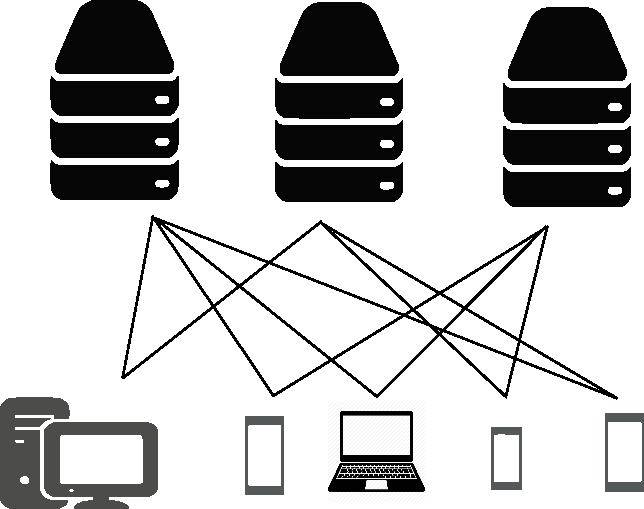
\includegraphics[width=0.6\linewidth]{server_sharing.pdf}
  \caption{An example server matching problem. A client is allowed to access only one server. The line illustrates that the corresponding server is within the client's strategy space.}
\label{server_sharing}
\end{figure}

Following the description in Section~\ref{congsetion_game}, we formulate the congestion game for this problem, 
\begin{itemize}
\item The clients constitute the players in the game $\mathcal{N}$, and the collection of servers $\mathcal{M}_i$ is the strategy space for player $i\in \mathcal{N}$.
\item The cost of a player in the game is equivalent to the latency experienced by the client in the problem.
If we denote the delay happens on the server $\alpha$ as $d_{\alpha}(n)$, where $n$ is the number of clients accessing the server, then the delay (cost) for a client (player) $i$ is $d_{\alpha}(n_r(\sigma))$, where $n_r(\sigma)$, $r\in \sigma_i$ is the number of clients using the server $r$.
\item As each user is allowed to use on server, this is a singleton congestion game according to Definition~\ref{background:singleton}.
\end{itemize}

\textit{Solution}: The solution for clients to match the servers is explicitly given by the proof of~\ref{background:polynomialConvergence}.
When the clients adopt best response strategy, \ie each player chooses the server which causes it the shortest delay with respect to other clients' choices, after a number of updates on the servers, the system reaches at NE, \ie the players cease to switch as they have the shortest delay in that state of NE. 
According to Theorem~\ref{background:finiteImprovement} and~\ref{background:polynomialConvergence}, the algorithm converges at Nash equilibrium after maximal $nm$ times of best responses.
%More formally, this corresponding congestion game is composed of players (the self-interested clients) and resources (servers), where players are allowed to choose one certain resources to use. 
%There is cost (latency) generated on a resource for the players who use that resource, and the cost is monotonic increasing with the number of players using it. 
%As congestion game permits convergence when every players in turn adopt the strategy which leads to a better utility.



%Thus in server matching problem, when clients in turn choose a permissible server with a smaller predicted latency, then after finite number of steps, no client has motivation to switch any more, and we reach a NE.

%If every player greedily searches the allowed resources to decrease its cost, the dynamics will cease in Nash equilibrium, where no player has motivation to adopt a new set of resources unilaterally. 




\subsection{Variants of Congestion Game}
In the congestion game we have introduced in Section ~\ref{congsetion_game}, the cost caused on one resource is function of the number of players using that resource.
In some variants of congestion game, the cost is decided by some other factors.
In \textit{player specific congestion game}, different players may have different delay functions.
As to \textit{weighted congestion game}, different players may have different impacts on the delays of the resources they allocate, in other words, there is a weight for every player, and the congestion on a resource is the total weight of all players using that resource.

As to neither player specific congestion game nor weighted congestion game, the finite converge does not hold anymore.
But there exits NE for both of Player specific congestion game and weighted congestion game when they are singleton congestion game~\cite{Milchtaich1996111, FKKMS02}.
When these variant of congestion game are not singleton ones, \cite{Ackermann06purenash} points that NE exists when the strategy space of players are matroid.








\section{Optimization}

A variety of problems in CRN are formulated and solved by constrained optimization~\cite{cacao_ca_2011, fuzzy_decision_09, resourceAllocation_imperfectSensing_2012}.
As to a player in a game, given the strategies of other players $\sigma_{-i}$, its utility $u_i$ is a function of its own strategy $\sigma_i$, then the maximization of its payoff or minimization of its cost becomes one optimization problem.
Thus, one game comprises $n$ such optimization problems in total.

Table~\ref{opt_table} summarizes the commonly proposed objectives, involved resources and constraints in the optimization problems in the domain of wireless communication.
Part of the contents in the table refers \cite{Han:2008:RAW:1457343}.
As to CRN, the interference caused by secondary users on primary users is usually formulated into constraints, which distinguishes the problems in CRN from that in traditional wireless networks. 

Convexity is a pursued property in optimization problem solving~\cite{Boyd:2004:CO:993483}.
As to a convex optimization \ie minimizing a convex objective function over a convex constraint set, a local optimum is also a global optimum and the duality gap is zero, and there are provably polynomial-time algorithms to solve the convex optimization, \ie interior-point methods. 
It is common to conduct optimization in centralized manner in small scale network, but in large scale network, centralized solution is infeasible for several reasons.
First, it is hard to obtain the information resides across the network, especially when the information is varying, \ie the spectrum availability at secondary users in CRN.
Second, it is hard for the centralized scheme to scale with the network~\cite{Palomar06atutorial}.

\subsection{Decomposition Methods}
The decomposition methods are originally proposed to solve very large optimization problems, but as a side effect, it also yields decentralized solution algorithms, which is important in many scenarios of wireless network~\cite{boyd2007notes}. 
In certain cases, decentralized solutions can be interpreted as a set of simple protocols which allow a collection of subsystems to coordinate so that to achieve global optimality.
%To design distributed algorithms on the basis of an optimization problem, we need to decompose the original problem.

\textit{Decomposition method} decomposes the original problem into distributively solvable subproblmes.
Specifically, the decomposition techniques includes \textit{primal decomposition} and \textit{dual decomposition}.
The primal decomposition decouples variables, \ie decomposes the original problem by allocating the available resources to each subproblem, and derived problem formulation is \textit{master problem}.
The dual decomposition solves the subproblems and decouples the constraints usually by forming Lagrangian~\cite{Bertsekas_99, Palomar06atutorial}.
There is communication between the master problem and the subproblems.
The communication is in the form of message passing which introduces overhead in the network.
In some cases, however, the communication is implicit in the system, \eg delay, packet error probability, as these quantities have physical meanings and can be implicitly measured without the need of explicit signaling.
The different ways to decouple the resources lead to different algorithms which have different characteristics of the amount of communication overhead and convergence properties.

We take the joint channel and power allocation problem in CRN~\cite{tachwali_opt_bandwidth_power_2013} as an example, to show how is one distributed algorithms obtained by decomposing the optimization problem.
To eliminate the impact of the coupling optimization variable, \ie channel and power levels, primal decomposition decomposes the original problem into two subproblems, channel allocation subproblem and power control subproblem. 
After solving the first subproblem of channel allocation, the power allocation subproblem is solved using dual-decomposition method, where the Lagrangian variables are calculated in decentralized manner with iterative sub-gradient algorithm.
Solving the two subproblems sequentially in one iteration, and the iterations cease when the change of the objective is below a given stopping criterion.
When the original problem is assumed convex, the derived distributed algorithms could have a provable con vergence to the global optimum.
The speed of convergence is difficult to quantify and will depend on how is the original problem is decomposed, \ie the number of levels in the decomposition, the amount of signaling, and the particular combination of numerical algorithms employed.




%When an optimization problem is convex, \ie to minimize a convex objective function over a convex constraint set, solving it very efficient. 
%More importantly, convexity means zero duality gap and thus enables distributed solutions through dual composition.


%When the problems involve channel allocation or modulation decision, binary variables need to be introduced in the problem formulation and the problems are mixed integer non-linear programming problems. 
%These problems are NP-hard to solve general, and the computational complexity becomes unaffordable when the network size scales up.
%In this case, we need to decompose the problems.
%
%Many wireless resource allocation or management problems are formulated as constrained optimization problems.

\begin{sidewaystable}
\centering
\begin{tabular}{|L{4cm}|C{5cm}|C{5cm}|C{5cm}|}
\hline 
 & Parameters & Optimization goals & Constraints \\ 
\hhline{|=|=|=|=|}
Application layer & source-coding rate, buffer priority, packet arrival rate & minimal delay & base layer transmission, strict delay requirement \\ 
\hline 
Network layer & routing path & end to end delay/throughput & maximal hops, security concerns \\ 
\hline 
MAC layer & transmission frequency, transmission priorities & maximal overall throughput, minimal buffer overflow probability & contentions, time/frequency slot \\ 
\hline
Physical layer & transmission power, modulation, channel coding rate, spectrum bandwidth & minimal over power consumption, maximal throughput, minimal BER, maximize product of bandwidth of power~\cite{tachwali_opt_bandwidth_power_2013} & maximal transmission power, interference on licensed users, available channel coding rate \\ 
\hline
\end{tabular} 
\caption{Optimization problem of cognitive radio networks}
\label{opt_table} 
\end{sidewaystable}

%the available radio resources such as spectrum and transmission power are scarce, meanwhile, new services raise new requirements for these resources.

%The solutions to optimization problems can be categorized by their properties, \ie convex, linear, integer, or non-convex non-linear, etc.
%In this thesis, we make use of different solvers, \ie Lindo, Gurobi, to solve the formulated optimization problems in different categories.


%Optimization outputs the results with the global information.
%Optimization is implemented on one entity, thus it is naturally suitable in centralized scheme.
